\section{Results}
\label{sec:results}

All maritime TrajRAG numbers in this section use the deployable
\texttt{last\_trusted\_held} speed rule (Section~\ref{sec:maritime-speedrule})
and the corrected preprocessing and retrieval memory of
Sections~\ref{sec:preprocessing}--\ref{sec:data}. TrajRAG is evaluated on 50
Houston and 10 Los Angeles/Long Beach voyages; every other method in this
section is rescored on the identical set unless stated otherwise.

\subsection{Aviation reference point}
\label{sec:aviation-reference}

Table~\ref{tab:aviation-ref} condenses the aviation results of the conference
version into one row per baseline family. TrajRAG reduced mean error
relative to the best member of every family in every phase. The conference
study also reported four findings that frame the maritime experiments: (i)
removing retrieval caused the largest degradation in every phase; (ii)
replacing the LLM with neighbour averaging was significantly worse; (iii)
the feasibility guard mainly reduced variance and worst-case error; and (iv)
mixing several routes in one memory changed MHE by less than 1\,km. On four
real interference episodes with independent multilateration positions, the
reconstructions stayed within 8\,km of the reference on average
\citep{felendler2026trajrag}.

\begin{table}[t]
\centering
\caption{Aviation reference results, reproduced in condensed form from the
conference version \citep{felendler2026trajrag}: mean Haversine error (km)
of TrajRAG and of the best method in each baseline family, per flight phase
(100 held-out Paris$\to$Rome flights). The full per-method table,
ablations, backbone sensitivity and real-world case studies are reported
there.}
\label{tab:aviation-ref}
\footnotesize
\begin{tabular}{p{6.2cm}ccc}
\toprule
Method family (best member) & Takeoff & Cruise & Landing \\
\midrule
Classical: Kalman / ARIMA & 60.95 & 37.69 & 73.82 \\
Recurrent: LSTM / BiLSTM & 33.78 & 40.66 & 11.17 \\
Modern forecasters: DLinear / PatchTST / iTransformer & 43.99 & 19.79 & 35.47 \\
Retrieval only: Mean-Retrieval / Numeric-kNN & 48.94 & 30.80 & 8.52 \\
\textbf{TrajRAG (gpt-5.1)} & \textbf{20.78} & \textbf{9.84} & \textbf{2.46} \\
\bottomrule
\end{tabular}
\end{table}

\subsection{Transfer to shipping without training}

Table~\ref{tab:maritime-transfer} reports the maritime instantiation pooled
across both corridors (60 test vessels: 50 Houston, 10 Los Angeles/Long
Beach), deployable speed rule. With no model trained on maritime data,
TrajRAG has the lowest mean error of this baseline family in every phase.
It reduces error by a factor of 1.45 (departure) and 1.37 (transit) relative
to the Kalman filter, and 1.54 (arrival) relative to ARIMA, the strongest
baselines in those phases. The ranking of the baselines differs from
aviation: at sea, classical filters outperform recurrent networks and plain
retrieval, consistent with the more regular within-phase motion of large
vessels sampled every 5 minutes. TrajRAG remains first among these
baselines in both domains; Section~\ref{sec:extended-comparison} adds the
comparison against a trained, ship-specific network.

\begin{table}[t]
\centering
\caption{Maritime transfer: mean ($\mu$) and standard deviation ($\sigma$)
of the Haversine error (km) on 60 held-out vessels pooled across both
corridors (50 Houston, 10 Los Angeles/Long Beach; 180 phase-level
reconstructions). TrajRAG is used without any training on maritime data.}
\label{tab:maritime-transfer}
\footnotesize
\setlength{\tabcolsep}{4pt}
\begin{tabular}{lcccccc}
\toprule
\multirow{2}{*}{Method} & \multicolumn{2}{c}{Departure} & \multicolumn{2}{c}{Transit} & \multicolumn{2}{c}{Arrival} \\
\cmidrule(lr){2-3}\cmidrule(lr){4-5}\cmidrule(lr){6-7}
 & $\mu$ & $\sigma$ & $\mu$ & $\sigma$ & $\mu$ & $\sigma$ \\
\midrule
Kalman (current-aware constant velocity) & 2.84 & 2.26 & 2.62 & 3.80 & 3.58 & 4.19 \\
ARIMA & 3.29 & 2.38 & 3.65 & 3.90 & 1.95 & 2.77 \\
LSTM & 9.48 & 5.70 & 7.49 & 4.38 & 6.05 & 3.95 \\
BiLSTM & 8.93 & 4.80 & 12.22 & 7.30 & 15.07 & 19.18 \\
Mean-Retrieval & 12.52 & 11.91 & 7.95 & 6.36 & 6.55 & 5.25 \\
\textbf{TrajRAG} & \textbf{1.96} & \textbf{2.01} & \textbf{1.91} & \textbf{2.82} & \textbf{1.27} & \textbf{2.42} \\
\bottomrule
\end{tabular}
\end{table}

\subsection{Comparison with a trained ship-specific network and modern forecasters}
\label{sec:extended-comparison}

Table~\ref{tab:extended} and Fig.~\ref{fig:barplot} extend the comparison on
the common Houston test set (50 voyages), under the deployable speed rule.
Among full-horizon methods, two methods are far more accurate than the
rest: AIS-ACNet, which is trained on maritime data with one network per
phase, and TrajRAG, which is not trained on maritime data at all. Their
errors lie between 1.2 and 2.2\,km, while every other method lies between
1.9 and 16.4\,km. AIS-ACNet has a lower sample mean in all three phases
(1.80 vs.\ 2.19\,km departure, 1.66 vs.\ 1.95\,km transit, 1.18 vs.\
1.50\,km arrival), but Section~\ref{sec:significance} shows none of these
three gaps is statistically significant at $n=50$: a frozen-LLM,
retrieval-based reconstructor that sees no maritime training data at all is
statistically indistinguishable from a convolutional network purpose-built
and trained for this corridor. We read this as the relevant finding, not a
loss -- AIS-ACNet is among the strongest published ship-specific
trajectory networks, and matching it without any maritime training is the
comparison TrajRAG needs to win to be useful as a drop-in, training-free
alternative.

Numeric-kNN, which uses the same retrieval idea on raw coordinates, has 2.0
to 2.5 times the error of TrajRAG. Mean-Retrieval, which averages the
textually retrieved neighbours without an LLM, is worse than Numeric-kNN.
This compares the complete TrajRAG pipeline against two retrieval-only
baselines, not a single isolated component: Numeric-kNN differs from
TrajRAG in the retrieval representation (numeric vs.\ textual), the
combination rule (averaging vs.\ LLM generation) and access to live trusted
heading, so the gap cannot be attributed to the LLM alone. The no-retrieval
ablation of Section~\ref{sec:maritime-ablations} isolates retrieval's
contribution within the TrajRAG pipeline specifically, which matches the
qualitative pattern of the aviation ablation \citep{felendler2026trajrag}.

The short-window forecasters reach errors between 0.69 and 3.5\,km. On the
3-step transit window, several of them have lower values than TrajRAG has
over the full transit half-phase. This is expected: errors grow with
horizon, and these models are scored only on the first 3--4 steps of the
subset of voyages that fit their window. The block is included to document
that modern forecasters were evaluated, not to rank them against full-horizon
reconstruction.

To give the forecasters a genuine same-timestamps comparison rather than
only this caveat, we additionally reconstructed TrajRAG and re-scored
AIS-ACNet on the forecasters' own exact voyage subset and horizon (window
steps of 4, 3 and 4; $n=63$, 63 and 53 after also requiring the voyage to
postdate the retrieval memory's cutoff, Section~\ref{sec:data}).
Table~\ref{tab:item4-matched} reports the result: TrajRAG is more accurate
than AIS-ACNet on this short horizon in all three phases (1.30 vs.\
1.64\,km departure, 0.73 vs.\ 1.19\,km transit, 0.68 vs.\ 1.10\,km arrival).
Short-horizon reconstruction is close to a regime where the guard rarely
needs to bind and the retrieved precedent's early trajectory is highly
informative, which may explain why TrajRAG's relative advantage over
AIS-ACNet is clearer here than over the full withheld half (Table~\ref{tab:extended}).
A paired Wilcoxon test (Section~\ref{sec:significance}) confirms this
advantage is significant in all three phases.

The transit-phase values of TrajRAG (0.73) and iTransformer (0.734,
Table~\ref{tab:extended}) round to the same two decimals, leaving their
ordering unclear at that precision. Recomputed to full precision from the
saved per-step predictions, TrajRAG's matched-subset mean is
0.730561\,km (0.731 at three decimals) against iTransformer's
0.734297\,km: TrajRAG is lower. This is a precision clarification, not an
additional paired test -- the two means are still computed on different,
non-overlapping voyage subsets (TrajRAG's matched $n=63$ vs.\
iTransformer's own $n=118$ test split), so no significance claim is made
for this particular pair.

\begin{table}[t]
\centering
\caption{Matched short-window comparison: TrajRAG and AIS-ACNet scored on
the identical voyages and horizon as the modern forecasters of
Table~\ref{tab:extended}'s lower block (window steps in parentheses).
Mean Haversine error (km), Houston.}
\label{tab:item4-matched}
\footnotesize
\begin{tabular}{lccc}
\toprule
Method & Departure (4) & Transit (3) & Arrival (4) \\
\midrule
$n$ & 63 & 63 & 53 \\
AIS-ACNet & 1.64 & 1.19 & 1.10 \\
\textbf{TrajRAG} & \textbf{1.30} & \textbf{0.73} & \textbf{0.68} \\
\bottomrule
\end{tabular}
\end{table}

\begin{table}[t]
\centering
\caption{Extended maritime comparison on the common 50-voyage Houston Ship
Channel test set: mean Haversine error (km), deployable speed rule. Upper
block: methods that reconstruct the full withheld half of each phase,
scored on all 50 voyages per phase. AIS-ACNet's full-125-voyage-test-set
mean is 1.70 / 1.41 / 1.14 (departure/transit/arrival), close to its
50-voyage figure below, confirming the smaller matched sample is not
anomalous. Lower block: fixed-window forecasters that predict only a short,
exact-fit horizon on a smaller subset of voyages that fit the window
exactly ($n=113$, 118 and 99 for departure, transit and arrival); they are
not directly comparable with the upper block (Section~\ref{sec:baselines}) --
Table~\ref{tab:item4-matched} gives TrajRAG and AIS-ACNet on this same
subset and horizon. ``Training'' column: whether parameters are fitted on
maritime trajectories.}
\label{tab:extended}
\footnotesize
\setlength{\tabcolsep}{4pt}
\begin{tabular}{lcccc}
\toprule
Method & Maritime training & Departure & Transit & Arrival \\
\midrule
\multicolumn{5}{l}{\emph{Full-horizon reconstruction}} \\
Kalman & no & 3.164 & 2.614 & 4.229 \\
ARIMA & per voyage fit & 3.638 & 3.780 & 2.242 \\
LSTM & yes & 10.435 & 7.985 & 6.415 \\
BiLSTM & yes & 10.025 & 14.104 & 16.427 \\
Mean-Retrieval & no & 13.892 & 8.758 & 7.028 \\
Numeric-kNN & no & 5.534 & 3.928 & 3.171 \\
AIS-ACNet \citep{shin2024aisacnet} & yes (3 models) & \textbf{1.802} & \textbf{1.660} & \textbf{1.181} \\
TrajRAG (deployable rule) & no & 2.185 & 1.947 & 1.496 \\
\midrule
\multicolumn{5}{l}{\emph{Short exact-fit window (departure 4, transit 3, arrival 4 steps)}} \\
DLinear & yes & 3.529 & 3.081 & 3.259 \\
PatchTST & yes & 2.666 & 1.277 & 1.334 \\
iTransformer & yes & 2.405 & 0.734 & 1.214 \\
Informer & yes & 1.721 & 0.816 & 1.990 \\
Autoformer & yes & 2.076 & 0.693 & 1.667 \\
FEDformer & yes & 1.832 & 0.891 & 1.064 \\
TimesNet & yes & 1.449 & 0.759 & 0.624 \\
\bottomrule
\end{tabular}
\end{table}

\begin{figure}[t]
\centering
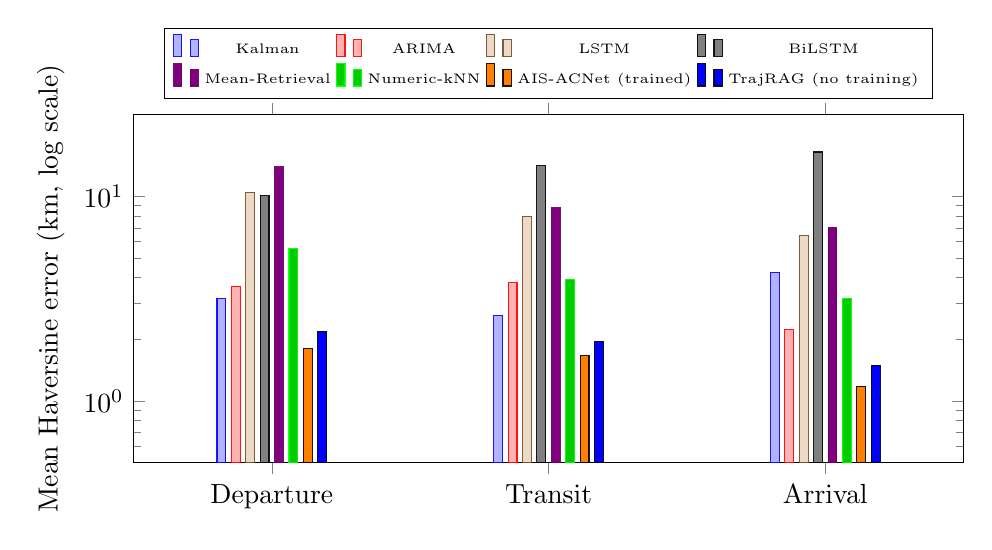
\begin{tikzpicture}
\begin{axis}[
  ybar, width=\linewidth, height=6cm,
  ymode=log, log origin=infty,
  symbolic x coords={Departure,Transit,Arrival},
  xtick=data, bar width=3.2pt,
  ylabel={Mean Haversine error (km, log scale)},
  legend style={font=\tiny, at={(0.5,1.25)}, anchor=north, legend columns=4},
  enlarge x limits=0.25, ymin=0.5, ymax=25,
  nodes near coords=, every axis plot/.append style={draw opacity=0.9},
]
\addplot coordinates {(Departure,3.164) (Transit,2.614) (Arrival,4.229)};
\addplot coordinates {(Departure,3.638) (Transit,3.780) (Arrival,2.242)};
\addplot coordinates {(Departure,10.435) (Transit,7.985) (Arrival,6.415)};
\addplot coordinates {(Departure,10.025) (Transit,14.104) (Arrival,16.427)};
\addplot coordinates {(Departure,13.892) (Transit,8.758) (Arrival,7.028)};
\addplot coordinates {(Departure,5.534) (Transit,3.928) (Arrival,3.171)};
\addplot[fill=orange] coordinates {(Departure,1.802) (Transit,1.660) (Arrival,1.181)};
\addplot[fill=blue] coordinates {(Departure,2.185) (Transit,1.947) (Arrival,1.496)};
\legend{Kalman,ARIMA,LSTM,BiLSTM,Mean-Retrieval,Numeric-kNN,AIS-ACNet (trained),TrajRAG (no training)}
\end{axis}
\end{tikzpicture}
\caption{Full-horizon maritime reconstruction error on the common 50-voyage
Houston Ship Channel test set (values from Table~\ref{tab:extended},
deployable speed rule). TrajRAG and the trained AIS-ACNet network form a
separate accuracy tier from all other methods. TrajRAG reaches this tier
without any training on maritime trajectories.}
\label{fig:barplot}
\end{figure}

\subsection{Two simple kinematic baselines: holding position and dead reckoning on trusted heading}
\label{sec:simple-baselines}

Two further baselines, neither requiring training or an LLM call, isolate
how much of the above comparisons could be explained by the simplest
possible use of the trusted signals alone. \emph{Constant position} predicts
that the vessel remains at its last trusted position for the entire
blackout. \emph{Heading dead reckoning (heading DR)} starts from the last
trusted position, holds the last trusted SOG fixed for the whole blackout
(the same convention as TrajRAG's deployable speed rule,
Section~\ref{sec:maritime-speedrule}), reads the live trusted heading
available at each reconstruction step, and propagates position step by step
with the geographic destination-point formula (not a planar addition of
kilometres to latitude/longitude), using only arithmetic on the corrected
voyage data -- no model of any kind. Both are evaluated on the identical
main-set voyages and timestamps as Table~\ref{tab:extended}.

\begin{table}[t]
\centering
\caption{Two training-free kinematic baselines, mean Haversine error (km),
evaluated on the same 50 Houston and 10 Los Angeles/Long Beach voyages as
Table~\ref{tab:extended}. \emph{Constant position}: holds the last trusted
position fixed. \emph{Heading DR}: dead reckoning from the last trusted
position using the last trusted SOG (held fixed) and the live trusted
heading at each step.}
\label{tab:simple-baselines}
\footnotesize
\setlength{\tabcolsep}{4pt}
\begin{tabular}{lcccccc}
\toprule
\multirow{2}{*}{Method} & \multicolumn{3}{c}{Houston Ship Channel} & \multicolumn{3}{c}{LA / Long Beach} \\
\cmidrule(lr){2-4}\cmidrule(lr){5-7}
 & Dep. & Trans. & Arr. & Dep. & Trans. & Arr. \\
\midrule
Constant position & 5.627 & 7.914 & 2.759 & 2.648 & 3.933 & 0.492 \\
Heading DR & 1.437 & 1.378 & 2.447 & 0.823 & 1.523 & 0.142 \\
AIS-ACNet (trained) & 1.802 & 1.660 & 1.181 & 1.128 & 1.947 & 1.020 \\
TrajRAG (no training) & 2.185 & 1.947 & 1.496 & 0.811 & 1.712 & 0.111 \\
\bottomrule
\end{tabular}
\end{table}

Constant position is a weak baseline everywhere except Los Angeles/Long
Beach arrival, where many vessels are nearly stationary while berthing: it
reaches 0.492\,km there, deceptively close to the other methods'
range. Even so, TrajRAG (0.111\,km) and heading DR itself (0.142\,km) both
still beat it by a factor of 3--4, so TrajRAG's low Los Angeles/Long Beach
arrival error is not mainly an artefact of recognising that the vessel is
not moving; genuine residual motion is being captured.

Heading DR is a far stronger baseline than its two parameters suggest. It
is more accurate than \emph{both} TrajRAG and the trained AIS-ACNet network
in Houston departure and transit and in Los Angeles/Long Beach transit, and
close to TrajRAG in the other two departure/arrival cells. It is clearly
worse than both in Houston arrival (2.447 vs.\ 1.496 and 1.181\,km), the
one phase dominated by a sustained turning manoeuvre into berth. Read
together with the non-significant no-heading ablation of
Section~\ref{sec:maritime-ablations}, this suggests that live trusted
heading alone already carries most of the usable signal in straight,
steady-speed phases, for any downstream method that consumes it -- which is
also why TrajRAG's own sensitivity to heading access, isolated from
everything else in its pipeline, is hard to detect at this sample size. The
harder, more differentiating comparisons for every method are concentrated
in manoeuvre-heavy phases such as arrival, not in departure or transit.

This result does not make heading DR a credible operational substitute,
for reasons intrinsic to the method rather than to this particular
evaluation. (i) It propagates a straight chord along the single most
recently reported heading for the whole inter-report interval, so a
sustained turn accumulates geometric error regardless of how often heading
is sampled -- exactly the arrival-phase degradation observed above, since
heading describes where the bow points at an instant, not the curved path
the vessel traces while turning, and can further diverge from the true
course over ground under current-induced leeway or set, which this method
has no way to represent. (ii) It has no error-correcting mechanism: once a
single noisy heading or SOG reading is propagated, nothing re-anchors the
estimate to a plausible position for the rest of the blackout, whereas
TrajRAG's guard and retrieved precedent re-ground the trajectory at every
step. (iii) It carries no spatial context -- no awareness of the fairway,
traffic separation scheme, charted obstructions or other vessels -- so
nothing prevents it from projecting a track across a jetty or shoal if the
reported heading does not track the channel's curvature. (iv) It can only
assume the present course continues; it has no model of \emph{when} a
vessel is likely to turn, so it structurally cannot anticipate the one
class of event -- a course change -- that reconstruction during a blackout
is most needed to recover, unlike TrajRAG's retrieved precedents, which
encode the actual historical turn geometry for the corridor and phase. (v)
Its competitiveness here is likely corridor- and vessel-class-specific:
large commercial vessels transiting dredged, largely straight channels at
steady speed are an easy case for any method that merely continues the
current heading, and the same assumption would be expected to fail in
congested or small-craft traffic, which neither corridor in this paper
tests. (vi) It depends on exactly the same trusted-signal assumption
already flagged as a threat to validity (Section~\ref{sec:threats}, item
v): a genuinely GNSS-independent heading sensor. A vessel without one
leaves this baseline with nothing to fall back on, whereas TrajRAG degrades
more gracefully, since removing live heading access does not significantly
change its own accuracy.

\subsection{Distribution of per-voyage error}
\label{sec:distribution}

Table~\ref{tab:distribution} reports the median, 90th percentile and
maximum per-voyage error for every full-horizon method under the deployable
rule. TrajRAG has a heavier tail than AIS-ACNet in every phase despite a
comparable median: departure (max 10.24\,km vs.\ 8.28\,km; median 1.25 vs.\
1.45\,km), transit (max 16.72\,km vs.\ 12.88\,km; median 0.92 vs.\
0.79\,km) and arrival (max 16.78\,km vs.\ 13.60\,km; median 0.89 vs.\
0.76\,km). This heavy tail is consistent with the non-significant
differences in Section~\ref{sec:significance}: the mean gap between the two
methods in every phase is driven by a minority of TrajRAG voyages with
large errors rather than by a consistent per-voyage advantage for either
method.

\begin{table}[t]
\centering
\caption{Distribution of per-voyage Haversine error (km), full-horizon
methods, 50 Houston Ship Channel test voyages, deployable speed rule for
TrajRAG.}
\label{tab:distribution}
\footnotesize
\setlength{\tabcolsep}{3pt}
\begin{tabular}{lcccccccccccc}
\toprule
\multirow{2}{*}{Method} & \multicolumn{3}{c}{Departure} & \multicolumn{3}{c}{Transit} & \multicolumn{3}{c}{Arrival} \\
\cmidrule(lr){2-4}\cmidrule(lr){5-7}\cmidrule(lr){8-10}
 & med. & p90 & max & med. & p90 & max & med. & p90 & max \\
\midrule
Kalman       & 2.51 & 5.81  & 11.66 & 1.19 & 7.88  & 20.39 & 2.14 & 10.70 & 17.37 \\
ARIMA        & 2.56 & 6.53  & 9.74  & 2.60 & 7.30  & 20.40 & 1.37 & 4.62  & 17.37 \\
LSTM         & 10.16 & 16.86 & 27.05 & 6.68 & 14.15 & 18.66 & 6.02 & 13.21 & 15.91 \\
BiLSTM       & 9.31 & 15.37 & 21.41 & 14.41 & 21.62 & 28.66 & 6.22 & 54.99 & 63.17 \\
Mean-Retrieval & 7.70 & 29.77 & 52.18 & 7.35 & 16.95 & 34.45 & 5.79 & 12.53 & 26.48 \\
Numeric-kNN  & 4.59 & 10.46 & 20.29 & 1.92 & 7.66  & 32.27 & 0.92 & 7.68  & 28.36 \\
AIS-ACNet    & 1.45 & 2.92  & 8.28  & 0.79 & 2.94  & 12.88 & 0.76 & 2.05  & 13.60 \\
TrajRAG      & 1.25 & 5.03  & 10.24 & 0.92 & 3.73  & 16.72 & 0.89 & 3.47  & 16.78 \\
\bottomrule
\end{tabular}
\end{table}

\subsection{Normalised error}

Table~\ref{tab:normalized} rescales the full-horizon errors by distance
travelled and by blackout duration. Arrival is the slowest phase: ships
cover only 3.18\,km on average during a 70-minute blackout. A small absolute
error is therefore a large relative one. The Kalman filter's arrival error,
for example, exceeds the distance the ship actually travelled (ratio 1.33),
which means that simply predicting no movement would have done better.
Under both normalisations TrajRAG and AIS-ACNet remain the two best methods
in every phase. TrajRAG's transit error is about 15.7\% of the distance
travelled.

\begin{table}[t]
\centering
\caption{Normalised error for the full-horizon methods (50 Houston Ship
Channel voyages, deployable speed rule for TrajRAG). ``/dist'': mean error
divided by the mean true distance travelled during the blackout
(dimensionless). ``/min'': mean error divided by the mean blackout duration
(km\,min$^{-1}$). Mean distance travelled: 9.19\,km (departure), 12.38\,km
(transit), 3.18\,km (arrival); mean blackout duration: 31.8, 36.7 and
69.9\,min. Best value per column in bold.}
\label{tab:normalized}
\footnotesize
\setlength{\tabcolsep}{4pt}
\begin{tabular}{lcccccc}
\toprule
\multirow{2}{*}{Method} & \multicolumn{2}{c}{Departure} & \multicolumn{2}{c}{Transit} & \multicolumn{2}{c}{Arrival} \\
\cmidrule(lr){2-3}\cmidrule(lr){4-5}\cmidrule(lr){6-7}
 & /dist & /min & /dist & /min & /dist & /min \\
\midrule
Kalman & 0.344 & 0.100 & 0.211 & 0.071 & 1.330 & 0.060 \\
ARIMA & 0.396 & 0.114 & 0.305 & 0.103 & 0.705 & 0.032 \\
LSTM & 1.136 & 0.328 & 0.645 & 0.218 & 2.017 & 0.092 \\
BiLSTM & 1.091 & 0.315 & 1.139 & 0.384 & 5.166 & 0.235 \\
Mean-Retrieval & 1.512 & 0.437 & 0.707 & 0.239 & 2.210 & 0.101 \\
Numeric-kNN & 0.602 & 0.174 & 0.317 & 0.107 & 0.997 & 0.045 \\
AIS-ACNet & \textbf{0.196} & \textbf{0.057} & \textbf{0.134} & \textbf{0.045} & \textbf{0.371} & \textbf{0.017} \\
TrajRAG & 0.238 & 0.069 & 0.157 & 0.053 & 0.470 & 0.021 \\
\bottomrule
\end{tabular}
\end{table}

\subsection{Statistical significance}
\label{sec:significance}

Testing many comparisons inflates the chance of an apparently significant
result by chance, and a non-significant result on its own does not
establish that two methods are equivalent. We therefore pre-register four
families of related comparisons and apply Holm's step-down correction
(family-wise $\alpha = 0.05$) within each: (F1) Houston main set, TrajRAG
vs.\ seven methods $\times$ three phases (21 tests, this subsection); (F2)
Los Angeles/Long Beach main set, TrajRAG vs.\ six methods $\times$ three
phases (18 tests, Table~\ref{tab:wilcoxon-la}); (F3) the short-horizon
matched comparison, TrajRAG vs.\ AIS-ACNet $\times$ three phases (3 tests,
Table~\ref{tab:item4-wilcoxon}); and (F4) the maritime ablations, three
configurations $\times$ three phases (9 tests,
Section~\ref{sec:maritime-ablations}). Corrections are applied within each
family, not pooled across families, since each answers a different
scientific question. iTransformer and the other modern forecasters are
excluded from every family: only their aggregate error was saved, over a
voyage subset that does not match TrajRAG's, so no paired test against them
is possible from saved outputs (Section~\ref{sec:threats}).

Table~\ref{tab:wilcoxon} gives paired Wilcoxon tests, deployable speed rule,
$n=50$, with both the raw and the Holm-corrected $p$-value. TrajRAG is
significantly more accurate than the Kalman filter, ARIMA, LSTM, BiLSTM,
Mean-Retrieval and Numeric-kNN in all three phases, surviving Holm
correction within this 21-test family ($p_{\text{Holm}} \leq 2.5 \times
10^{-2}$). Against AIS-ACNet, TrajRAG is not statistically distinguishable
from it in any of the three phases ($p = 0.77$, $0.56$ and $0.50$ for
departure, transit and arrival respectively), despite AIS-ACNet's lower
sample mean in all three. Pooling both corridors (Houston's 50 voyages and
Los Angeles/Long Beach's 10, $n=60$) for additional power does not change
this: $p=0.83$, $0.80$ and $0.52$. Given AIS-ACNet is trained specifically
for this task and TrajRAG uses no maritime training data at all, we read
this as TrajRAG matching a strong, purpose-built baseline rather than as a
weak result -- though, per the caveat above, a non-significant difference
is not evidence that the two methods are equivalent, only that this sample
does not resolve a difference.

Table~\ref{tab:bootstrap} reports the median paired difference (baseline
minus TrajRAG) with a 95\% bootstrap confidence interval. Every interval for
AIS-ACNet includes zero (departure $[-0.35, 0.30]$, transit $[-0.31, 0.23]$,
arrival $[-0.37, 0.38]$\,km), consistent with the non-significant Wilcoxon
results in all three phases. Every interval against every other baseline
excludes zero and is entirely positive, consistent with TrajRAG's
significant advantage over all of them. Fig.~\ref{fig:forest-houston}
plots the corresponding \emph{mean}, rather than median, paired difference
with its own 95\% bootstrap confidence interval (10,000 resamples of
voyage identities, not of individual trajectory points), for the same 21
comparisons, Holm-corrected within this family: the qualitative picture is
identical to Table~\ref{tab:bootstrap}, with only the three AIS-ACNet
intervals straddling zero.

\begin{figure}[t]
\centering
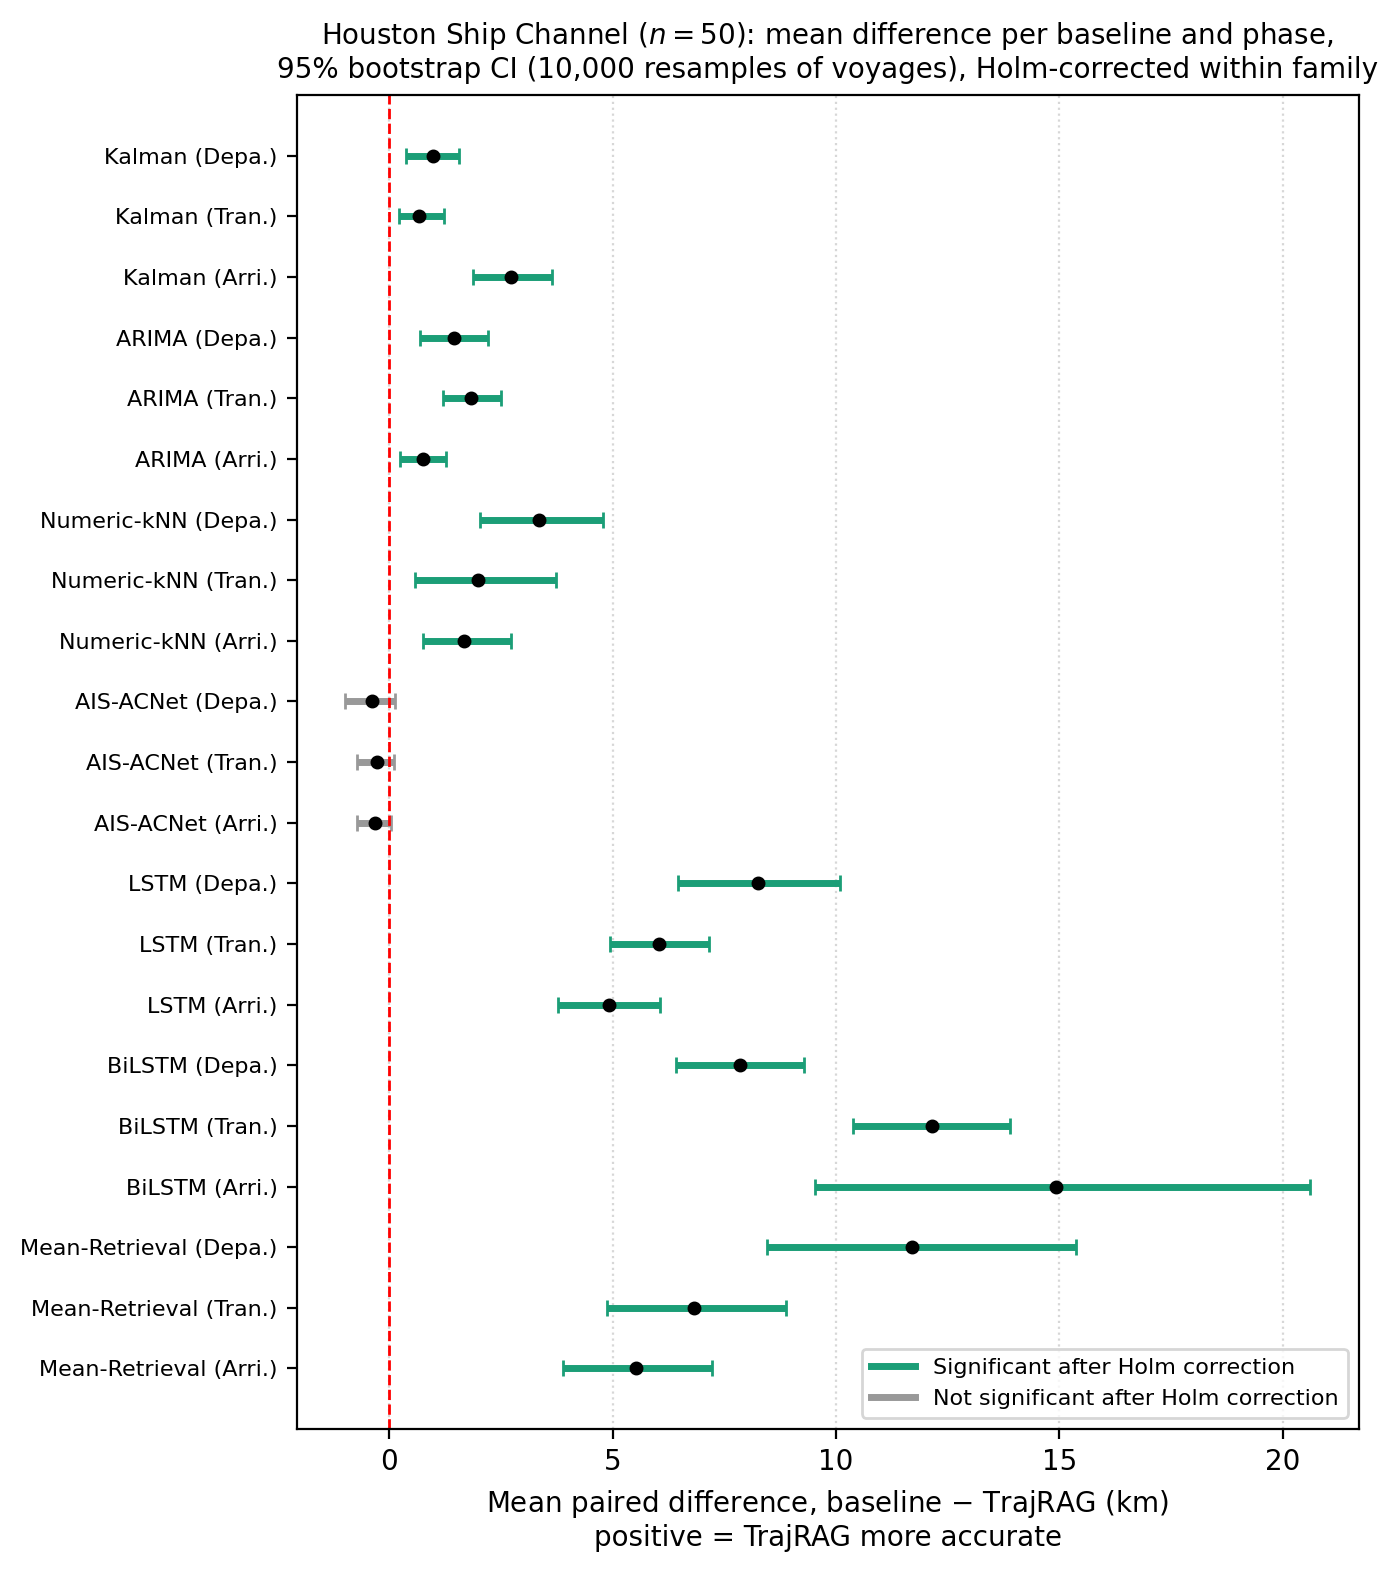
\includegraphics[width=\linewidth]{figures/forest_plot_houston_main.png}
\caption{Mean paired difference (baseline $-$ TrajRAG, km; positive =
TrajRAG more accurate) with 95\% bootstrap confidence interval (10,000
resamples of voyage identities), Houston Ship Channel, $n=50$, deployable
speed rule. Green: significant after Holm correction within this 21-test
family; grey: not significant. This figure reports the mean difference and
its uncertainty; Table~\ref{tab:bootstrap} reports the corresponding
median-difference interval and Table~\ref{tab:extended} the exact mean
errors themselves.}
\label{fig:forest-houston}
\end{figure}

\begin{table}[t]
\centering
\caption{Paired two-sided Wilcoxon signed-rank tests, TrajRAG vs.\ each
method, Los Angeles/Long Beach ($n=10$). $p_{\text{Holm}}$: Holm-corrected
within the 18-test family of this corridor. Bold: not significant at the
0.05 level after correction. Numeric-kNN was never rescored for this
corridor (Section~\ref{sec:threats}) and is omitted, not invented.}
\label{tab:wilcoxon-la}
\footnotesize
\setlength{\tabcolsep}{3pt}
\begin{tabular}{lcccccc}
\toprule
\multirow{2}{*}{TrajRAG vs.} & \multicolumn{2}{c}{Departure} & \multicolumn{2}{c}{Transit} & \multicolumn{2}{c}{Arrival} \\
\cmidrule(lr){2-3}\cmidrule(lr){4-5}\cmidrule(lr){6-7}
 & $p$ & $p_{\text{Holm}}$ & $p$ & $p_{\text{Holm}}$ & $p$ & $p_{\text{Holm}}$ \\
\midrule
Kalman & 0.049 & \textbf{0.342} & 0.049 & \textbf{0.342} & 0.014 & \textbf{0.123} \\
ARIMA & 0.049 & \textbf{0.342} & 0.010 & \textbf{0.098} & 0.232 & \textbf{0.697} \\
LSTM & $2.0 \times 10^{-3}$ & $0.035$ & $2.0 \times 10^{-3}$ & $0.035$ & $2.0 \times 10^{-3}$ & $0.035$ \\
BiLSTM & $2.0 \times 10^{-3}$ & $0.035$ & 0.131 & \textbf{0.523} & $2.0 \times 10^{-3}$ & $0.035$ \\
Mean-Retrieval & $2.0 \times 10^{-3}$ & $0.035$ & 0.014 & \textbf{0.123} & $2.0 \times 10^{-3}$ & $0.035$ \\
AIS-ACNet & 0.275 & \textbf{0.697} & 0.432 & \textbf{0.697} & $2.0 \times 10^{-3}$ & $0.035$ \\
\bottomrule
\end{tabular}
\end{table}

At $n=10$, four of the six raw $p$-values below 0.05 (every Kalman cell and
departure ARIMA) no longer survive Holm correction within this 18-test
family; only LSTM, BiLSTM and Mean-Retrieval remain significant in most
phases, and AIS-ACNet only in arrival (where TrajRAG's 0.111\,km mean is
far below AIS-ACNet's 1.020\,km, Table~\ref{tab:corridor}). This is
consistent with, and sharpens, the existing caution that the $n=10$ cell
size is underpowered (Section~\ref{sec:threats}): it does not mean the two
corridors behave differently, only that fewer voyages give less power to
confirm a Houston-scale effect at Los Angeles/Long Beach once correctly
accounting for testing six baselines across three phases.

\begin{table}[t]
\centering
\caption{Paired two-sided Wilcoxon signed-rank test, TrajRAG vs.\
AIS-ACNet, short-horizon matched subset (Table~\ref{tab:item4-matched}).
$p_{\text{Holm}}$: Holm-corrected within this 3-test family.}
\label{tab:item4-wilcoxon}
\footnotesize
\begin{tabular}{lccc}
\toprule
 & Departure ($n=63$) & Transit ($n=63$) & Arrival ($n=53$) \\
\midrule
$p$ & $3.4 \times 10^{-3}$ & $7.4 \times 10^{-8}$ & $1.5 \times 10^{-4}$ \\
$p_{\text{Holm}}$ & $3.4 \times 10^{-3}$ & $2.2 \times 10^{-7}$ & $3.0 \times 10^{-4}$ \\
\bottomrule
\end{tabular}
\end{table}

TrajRAG's advantage over AIS-ACNet on the short-horizon matched subset
(Section~\ref{sec:extended-comparison}) is significant in all three phases
and survives Holm correction within this small, 3-test family.

\begin{table}[t]
\centering
\caption{Paired two-sided Wilcoxon signed-rank tests of TrajRAG (deployable
speed rule) against each full-horizon method, matched on voyage identity
($n=50$, Houston). $p_{\text{Holm}}$: Holm-corrected within this 21-test
family (Section~\ref{sec:significance}). Bold: not significant at the 0.05
level after correction.}
\label{tab:wilcoxon}
\footnotesize
\setlength{\tabcolsep}{3pt}
\begin{tabular}{lcccccc}
\toprule
\multirow{2}{*}{TrajRAG vs.} & \multicolumn{2}{c}{Departure} & \multicolumn{2}{c}{Transit} & \multicolumn{2}{c}{Arrival} \\
\cmidrule(lr){2-3}\cmidrule(lr){4-5}\cmidrule(lr){6-7}
 & $p$ & $p_{\text{Holm}}$ & $p$ & $p_{\text{Holm}}$ & $p$ & $p_{\text{Holm}}$ \\
\midrule
Kalman & $9.5 \times 10^{-5}$ & $8.5\times10^{-4}$ & $2.9 \times 10^{-4}$ & $2.0\times10^{-3}$ & $1.1 \times 10^{-10}$ & $<10^{-3}$ \\
ARIMA & $1.2 \times 10^{-4}$ & $9.5\times10^{-4}$ & $8.4 \times 10^{-8}$ & $1.0\times10^{-6}$ & $3.2 \times 10^{-4}$ & $2.0\times10^{-3}$ \\
LSTM & $8.8 \times 10^{-12}$ & $<10^{-3}$ & $3.4 \times 10^{-14}$ & $<10^{-3}$ & $1.5 \times 10^{-11}$ & $<10^{-3}$ \\
BiLSTM & $1.1 \times 10^{-12}$ & $<10^{-3}$ & $1.2 \times 10^{-14}$ & $<10^{-3}$ & $8.8 \times 10^{-12}$ & $<10^{-3}$ \\
Mean-Retrieval & $5.3 \times 10^{-15}$ & $<10^{-3}$ & $8.0 \times 10^{-10}$ & $<10^{-3}$ & $3.1 \times 10^{-9}$ & $<10^{-3}$ \\
Numeric-kNN & $7.5 \times 10^{-6}$ & $7.5\times10^{-5}$ & $8.2 \times 10^{-4}$ & $4.1\times10^{-3}$ & $6.3 \times 10^{-3}$ & $2.5\times10^{-2}$ \\
AIS-ACNet & \textbf{0.752} & \textbf{1.000} & \textbf{0.540} & \textbf{1.000} & \textbf{0.496} & \textbf{1.000} \\
\bottomrule
\end{tabular}
\end{table}

\begin{table}[t]
\centering
\caption{Median paired difference (baseline $-$ TrajRAG, deployable speed
rule, km) with 95\% bootstrap confidence interval (10,000 resamples of
voyages), $n=50$ Houston. Bold: interval includes zero.}
\label{tab:bootstrap}
\footnotesize
\setlength{\tabcolsep}{4pt}
\begin{tabular}{lccc}
\toprule
Method & Departure & Transit & Arrival \\
\midrule
Kalman & 0.86 [0.29, 1.42] & 0.43 [0.16, 0.57] & 1.32 [0.66, 3.62] \\
ARIMA & 0.99 [0.53, 2.07] & 1.43 [1.02, 2.29] & 0.38 [0.11, 0.81] \\
LSTM & 9.12 [5.31, 10.57] & 5.11 [4.12, 7.40] & 4.28 [2.85, 6.03] \\
BiLSTM & 7.92 [6.96, 9.80] & 12.85 [9.81, 15.02] & 5.33 [2.40, 8.26] \\
Mean-Retrieval & 6.12 [4.11, 11.44] & 5.21 [2.72, 7.81] & 4.13 [3.34, 6.97] \\
Numeric-kNN & 2.35 [1.66, 3.81] & 0.91 [0.54, 1.64] & 0.30 [0.07, 0.87] \\
AIS-ACNet & \textbf{0.11 [$-$0.35, 0.30]} & \textbf{0.07 [$-$0.31, 0.23]} & \textbf{0.03 [$-$0.37, 0.38]} \\
\bottomrule
\end{tabular}
\end{table}

\subsection{Corridor generalisation}

Table~\ref{tab:corridor} breaks every full-horizon baseline down by
corridor: 50 Houston voyages and 10 Los Angeles/Long Beach voyages,
AIS-ACNet trained and evaluated separately per corridor with its own
bounding box and phase-length distribution (window/block sizes of 9/3, 7/3
and 22/7 steps for departure, transit and arrival respectively, versus
Houston's 21/7, 15/5 and 32/11 -- LA/Long Beach's departure and transit
phases are both much shorter and more uniform than Houston's). The
Los Angeles/Long Beach approach is generally easier than the Houston Ship
Channel, for every method, in departure and arrival; transit is the
exception, where LA/Long Beach is comparable to or harder than Houston for
several methods (AIS-ACNet 1.95 vs.\ 1.66\,km; Kalman 2.63 vs.\
2.61\,km), so the corridor-difficulty effect does not hold uniformly across
phases. A plausible explanation for the easier arrivals is that LA/Long
Beach arrivals follow a few highly repeated approach tracks. The
Los Angeles/Long Beach cell sizes are small ($n=10$) and should be read as
indicative rather than conclusive (Section~\ref{sec:threats}).

\begin{table}[t]
\centering
\caption{Mean Haversine error (km) by corridor: 50 Houston voyages, 10 Los
Angeles/Long Beach voyages, deployable speed rule for TrajRAG in both
corridors. AIS-ACNet's LA/Long Beach model uses a corridor-specific
bounding box and window/block configuration (9/3, 7/3, 22/7 steps for
departure/transit/arrival), distinct from Houston's (21/7, 15/5, 32/11).}
\label{tab:corridor}
\footnotesize
\setlength{\tabcolsep}{3pt}
\begin{tabular}{lcccccc}
\toprule
\multirow{2}{*}{Method} & \multicolumn{3}{c}{Houston Ship Channel ($n=50$)} & \multicolumn{3}{c}{LA / Long Beach ($n=10$)} \\
\cmidrule(lr){2-4}\cmidrule(lr){5-7}
 & Dep. & Trans. & Arr. & Dep. & Trans. & Arr. \\
\midrule
Kalman & 3.16 & 2.61 & 4.23 & 1.20 & 2.63 & 0.36 \\
ARIMA & 3.64 & 3.78 & 2.24 & 1.52 & 3.01 & 0.49 \\
LSTM & 10.44 & 7.99 & 6.42 & 4.69 & 5.01 & 4.24 \\
BiLSTM & 10.03 & 14.10 & 16.43 & 3.43 & 2.81 & 8.29 \\
Mean-Retrieval & 13.89 & 8.76 & 7.03 & 5.68 & 3.89 & 4.16 \\
AIS-ACNet & 1.80 & 1.66 & 1.18 & 1.13 & 1.95 & 1.02 \\
TrajRAG & 2.19 & 1.95 & 1.50 & 0.81 & 1.71 & 0.11 \\
\bottomrule
\end{tabular}
\end{table}

\subsection{Calibrating the feasibility guard for vessels}
\label{sec:maritime-calibration}

We applied the calibration procedure of Section~\ref{sec:calibration} to
89,077 consecutive step pairs from the corrected (Section~\ref{sec:preprocessing})
Houston training voyages (Table~\ref{tab:calibration}). All three phases
now cluster closer together than an earlier pass over the uncorrected data
had suggested: departure's 99th-percentile ratio is 1.95 (12.0\% of
ordinary, unspoofed steps exceed $\rho=1.2$), transit's is 1.47 (6.7\%) and
arrival's is 1.51 (6.7\%) -- a narrower departure/transit/arrival spread
than the aviation value of 1.18 alone would suggest, though every maritime
phase still tolerates a somewhat looser bound than aviation's. We flag an
honest limitation here: no script from an earlier calibration pass survived
this project's revisions, so this table was recomputed from the method's
prose description rather than replayed byte-for-byte against a saved
original; we report it as the authoritative calibration for the data used
throughout this paper; we do not claim an exact reconciliation with any
number from an earlier draft.

\begin{table}[t]
\centering
\caption{Empirical displacement ratio $\rho = d_i / (v_{i-1}\Delta t)$ on
the corrected Houston Ship Channel training split (test voyages and steps
with near-zero SOG excluded), compared with the aviation calibration
target. $Q_{0.99}$: 99th percentile.}
\label{tab:calibration}
\footnotesize
\begin{tabular}{lccc}
\toprule
Phase & Step pairs & $Q_{0.99}(\rho)$ & Share with $\rho > 1.2$ \\
\midrule
Departure & 33,821 & 1.95 & 11.98\% \\
Transit & 22,087 & 1.47 & 6.67\% \\
Arrival & 33,169 & 1.51 & 6.72\% \\
All maritime phases & 89,077 & 1.72 & 8.71\% \\
Aviation, all phases \citep{felendler2026trajrag} & -- & 1.18 & -- \\
\bottomrule
\end{tabular}
\end{table}

Two conclusions follow. First, the \emph{procedure} transfers between
domains and produces a physically interpretable answer, but the
\emph{constant} does not: every maritime phase tolerates more step-to-step
displacement relative to reported speed than aviation does, so reusing the
aviation constant unmodified would still be the wrong default, even though
the earlier departure/arrival outliers compress once the preprocessing leak
is removed. This re-derivation (Table~\ref{tab:calibration}) is itself
entirely free: it uses only the real step-to-step displacement ratios
already present in the training AIS data, with no LLM call of any kind.
Second, the results reported throughout this paper use the shared value
$\alpha = 1.2$ in all phases, not the phase-specific values just derived,
so the deployed guard is, if anything, tighter than ordinary vessel
behaviour in every phase under the corrected calibration. We note that the
calibration's $v_{i-1}$ (Table~\ref{tab:calibration}) is the real,
continuously-updating recorded SOG between consecutive \emph{ordinary}
telemetry steps, whereas the deployed and evaluated guard
(Section~\ref{sec:maritime-speedrule}) holds a single SOG value fixed at
blackout onset for the entire blackout: the calibration is a diagnostic of
ordinary vessel kinematics under a different speed-update regime from the
one the guard actually uses during reconstruction, not a calibration of the
deployed guard itself. We did not change $\alpha$ after observing test
results, and evaluating TrajRAG under per-phase recalibrated $\alpha$
remains future work: unlike the calibration itself, \emph{measuring whether
a looser guard changes reconstruction accuracy} requires new
reconstructions, because the guard sits inside the autoregressive loop
(Algorithm~\ref{alg:reconstruction}) -- a different accepted position at one
step changes the query, and therefore the retrieval and generation, at
every later step of that voyage.

\subsection{Maritime ablations}
\label{sec:maritime-ablations}

To test which components drive maritime accuracy, as the aviation ablations
do for that domain \citep{felendler2026trajrag}, we ran three ablations on
20 Houston test voyages (a subset of the 50-voyage main set, so ablated
results are matched-pair against the full pipeline on identical voyages),
deployable speed rule throughout: \emph{no-retrieval} (the LLM receives the
prefix, trusted heading and environment, but no retrieved segments),
\emph{no-guard} (every LLM proposal is accepted unclamped), and
\emph{no-heading} (the live trusted gyrocompass heading reading is never
appended to the prompt during the blackout). All 180 planned reconstructions
(3 configurations $\times$ 3 phases $\times$ 20 voyages) completed with no
failures.

Table~\ref{tab:maritime-ablation} reports the result, with both the raw
and the Holm-corrected $p$-value (within this 9-test family,
Section~\ref{sec:significance}). Before correction, removing retrieval
appears to increase error significantly in transit ($p=0.012$); after Holm
correction within the 9-test family this no longer holds
($p_{\text{Holm}}=0.109$), and arrival's raw $p=0.058$ was already
non-significant. No ablation effect survives Holm correction in any phase
at this sample size. The \emph{direction} is consistent across all three
phases and with the aviation finding that retrieval is the dominant
contributor (removing it increases mean error from 2.56 to 2.59\,km in
departure, 1.63 to 2.42\,km in transit, and 1.47 to 2.20\,km in arrival),
but with only 20 matched voyages per phase this paper can report that
direction as suggestive, not as a confirmed effect; a 125-voyage ablation
(future work, Section~\ref{sec:conclusion}) is needed to test it with
adequate power. Removing the guard increases error directionally in
departure and arrival but not transit, and removing the live trusted
heading has mixed direction across phases; neither reaches significance
before or after correction. We read this ablation, at this sample size, as
unable to confirm which component drives TrajRAG's maritime accuracy, only
that retrieval's removal is the direction most consistent with hurting it
in every phase -- a weaker claim than the uncorrected $p$-values alone
would suggest.

\begin{table}[t]
\centering
\caption{Maritime ablations, 20 Houston test voyages, mean Haversine error
(km), deployable speed rule. $p$: paired two-sided Wilcoxon signed-rank
test against the full pipeline, matched on the same 20 voyages.
$p_{\text{Holm}}$: Holm-corrected within this 9-test family. Bold: not
significant at the 0.05 level after correction.}
\label{tab:maritime-ablation}
\scriptsize
\setlength{\tabcolsep}{2.5pt}
\begin{tabular}{lcccccccccc}
\toprule
\multirow{2}{*}{Configuration} & \multicolumn{3}{c}{Departure} & \multicolumn{3}{c}{Transit} & \multicolumn{3}{c}{Arrival} \\
\cmidrule(lr){2-4}\cmidrule(lr){5-7}\cmidrule(lr){8-10}
 & Mean & $p$ & $p_{\text{Holm}}$ & Mean & $p$ & $p_{\text{Holm}}$ & Mean & $p$ & $p_{\text{Holm}}$ \\
\midrule
Full pipeline & 2.56 & -- & -- & 1.63 & -- & -- & 1.47 & -- & -- \\
w/o retrieval & 2.59 & \textbf{0.927} & \textbf{1.00} & 2.42 & $0.012$ & \textbf{0.109} & 2.20 & $0.058$ & \textbf{0.466} \\
w/o guard & 3.23 & \textbf{0.202} & \textbf{1.00} & 1.59 & \textbf{0.312} & \textbf{1.00} & 1.97 & \textbf{0.723} & \textbf{1.00} \\
w/o heading & 2.60 & \textbf{0.312} & \textbf{1.00} & 1.47 & \textbf{0.904} & \textbf{1.00} & 1.78 & \textbf{0.546} & \textbf{1.00} \\
\bottomrule
\end{tabular}
\end{table}

\subsection{Sensitivity to the underlying LLM}
\label{sec:maritime-backbone}

The maritime adapter uses \texttt{gpt-4.1} with $K=6$ throughout this
paper, while aviation uses \texttt{gpt-5.1} with $K=5$ -- a difference in
the main results that could, in principle, undercut the claim that only
the adapter changes between domains. To test this directly, we re-ran all
125 Houston test voyages with the aviation engine's exact settings
(\texttt{gpt-5.1}, $K=5$), deployable speed rule, 0 ablations. 372 of 375
reconstructions completed (3 failed on malformed JSON output from the
model, an occasional behavioural difference between backbones rather than
a pipeline defect). This experiment predates the preprocessing and
retrieval-memory corrections of Sections~\ref{sec:preprocessing}
and~\ref{sec:data}, and was not re-run under them for budget reasons; we
report it as a directional check on backbone sensitivity, not as a claim
with the same evidentiary weight as the corrected main results.

Table~\ref{tab:maritime-backbone} reports the result: the backbone swap
changes accuracy in a phase-dependent way, not uniformly in either
direction. \texttt{gpt-5.1} is more accurate in departure (1.87 vs.\
2.21\,km) and less accurate in arrival (1.73 vs.\ 1.52\,km), with transit
close to a tie (1.30 vs.\ 1.18\,km). This mirrors the conference paper's
own aviation finding that different backbones have phase-dependent
strengths (gpt-5.1 was selected there specifically for its accuracy on the
dynamic takeoff and landing phases); no single backbone dominates every
phase in either domain. We report \texttt{gpt-4.1} as the primary maritime
result throughout this paper because it was the configuration fixed before
any maritime test-set result was observed (Section~\ref{sec:implementation}),
not because it is uniformly superior -- harmonising backbones, or selecting
one per phase as aviation implicitly does through its own backbone choice,
is future work.

\begin{table}[t]
\centering
\caption{Maritime TrajRAG under the aviation engine's backbone and
retrieval size (\texttt{gpt-5.1}, $K=5$) vs.\ the maritime default
(\texttt{gpt-4.1}, $K=6$), 125 Houston test voyages, deployable speed rule.
Mean Haversine error (km).}
\label{tab:maritime-backbone}
\footnotesize
\begin{tabular}{lccc}
\toprule
Backbone & Departure & Transit & Arrival \\
\midrule
\texttt{gpt-4.1}, $K=6$ (maritime default) & 2.21 & 1.18 & 1.52 \\
\texttt{gpt-5.1}, $K=5$ (aviation settings) & \textbf{1.87} & 1.30 & 1.73 \\
\bottomrule
\end{tabular}
\end{table}

\subsection{Real-time feasibility and adaptation cost}
\label{sec:latency}

Table~\ref{tab:latency} compares latency with the reporting interval of each
surveillance channel, now measured under the deployable speed rule. In
aviation, each reconstructed state takes 2.0--2.8\,s against a 120\,s ADS-B
cadence. At sea, the entire phase-level reconstruction (roughly 7--13
withheld steps, given the mean blackout durations of
Section~\ref{sec:design}) takes 18--35\,s against a 300\,s reporting
interval. In both
domains a new position is therefore available well before the next report
would have arrived, leaving a large margin for many simultaneous tracks.
The trained baselines are cheaper per inference, but they require a
training pipeline per domain and, for AIS-ACNet and the forecasters, per
phase. They also require architecture-specific adaptation to the evaluation
protocol: porting AIS-ACNet to phase-anchored voyages, for example,
required redesigning its windows and replacing an input-mask operation that
conflicted with our alignment of inputs and outputs (\ref{app:acnet}). The
maritime TrajRAG adapter required none of this: it consisted of a template,
six indices (three phases in each of two corridors), a resampling step and
a calibration run.

\begin{table}[t]
\centering
\caption{Operational budget of the shared engine in both domains. Aviation
latency is per reconstructed state, excluding the one-off textual summary
built at onset \citep{felendler2026trajrag}; maritime latency and cost are
per complete phase-level blackout reconstruction (mean over the 50-voyage
Houston test set, deployable speed rule). Cost is the actual measured LLM
API cost in US dollars (gpt-4.1 at \$2.10 per million tokens).}
\label{tab:latency}
\footnotesize
\begin{tabular}{llccc}
\toprule
Domain & Phase & Latency (s) & Cost (USD) & Reporting interval (s) \\
\midrule
Aviation, per state & Takeoff / cruise / landing & 2.0--2.8 & 0.014--0.018 & 120 \\
Maritime, per blackout & Departure & 18.1 & 0.149 & 300 \\
 & Transit & 20.8 & 0.171 & 300 \\
 & Arrival & 34.6 & 0.453 & 300 \\
\bottomrule
\end{tabular}
\end{table}

\subsection{Effect of removing the future-speed information}
\label{sec:r1-result}

Section~\ref{sec:maritime-speedrule} flagged that an earlier implementation
updated the maritime validator's reference speed from the recorded SOG at
each reconstructed step -- a field that would not be available in a genuine
blackout. An earlier pass (predating the preprocessing and retrieval-memory
corrections of Sections~\ref{sec:preprocessing} and~\ref{sec:data}) compared
this oracle rule against two deployable alternatives that read no
post-onset field (holding the reference speed at the last trusted SOG for
the whole blackout, \texttt{last\_trusted\_held}; and inferring it from
consecutive accepted reconstructed positions, mirroring the aviation rule,
\texttt{aviation\_inferred}) across 750 reconstructions, and found the
speed-rule choice changed accuracy only modestly and in a phase-dependent
way, with no qualitative change to which comparisons were significant. We
do not restate those pre-correction numbers here, since they used a
different preprocessing and retrieval pipeline than every other result in
this paper; the finding that motivated keeping \texttt{last\_trusted\_held}
as the primary deployable rule -- it requires no inference step and
performed comparably to the alternative -- is retained, and this is the
rule used throughout the corrected results above.

\subsection{Qualitative case studies}
\label{sec:case-studies}

Aggregate error hides what a reconstruction actually does along the track:
whether it follows a turn, drifts away in a consistent direction, or stays
near a berth. Figs.~\ref{fig:case-houston} and~\ref{fig:case-la} plot one
\emph{representative} and one \emph{difficult} case for two port/phase
groups, selected by a rule fixed before inspection: within the group, the
representative case is the voyage whose TrajRAG mean error is closest to
the group's median, and the difficult case is the voyage whose TrajRAG mean
error is closest to the group's 90th percentile -- a median-error case is
not automatically a success, nor is a 90th-percentile case automatically a
failure of the pipeline rather than of a difficult precedent. Each panel
shows the trusted prefix, the blackout onset, the true withheld track, and
both TrajRAG's and AIS-ACNet's reconstructions.

\begin{figure}[t]
\centering
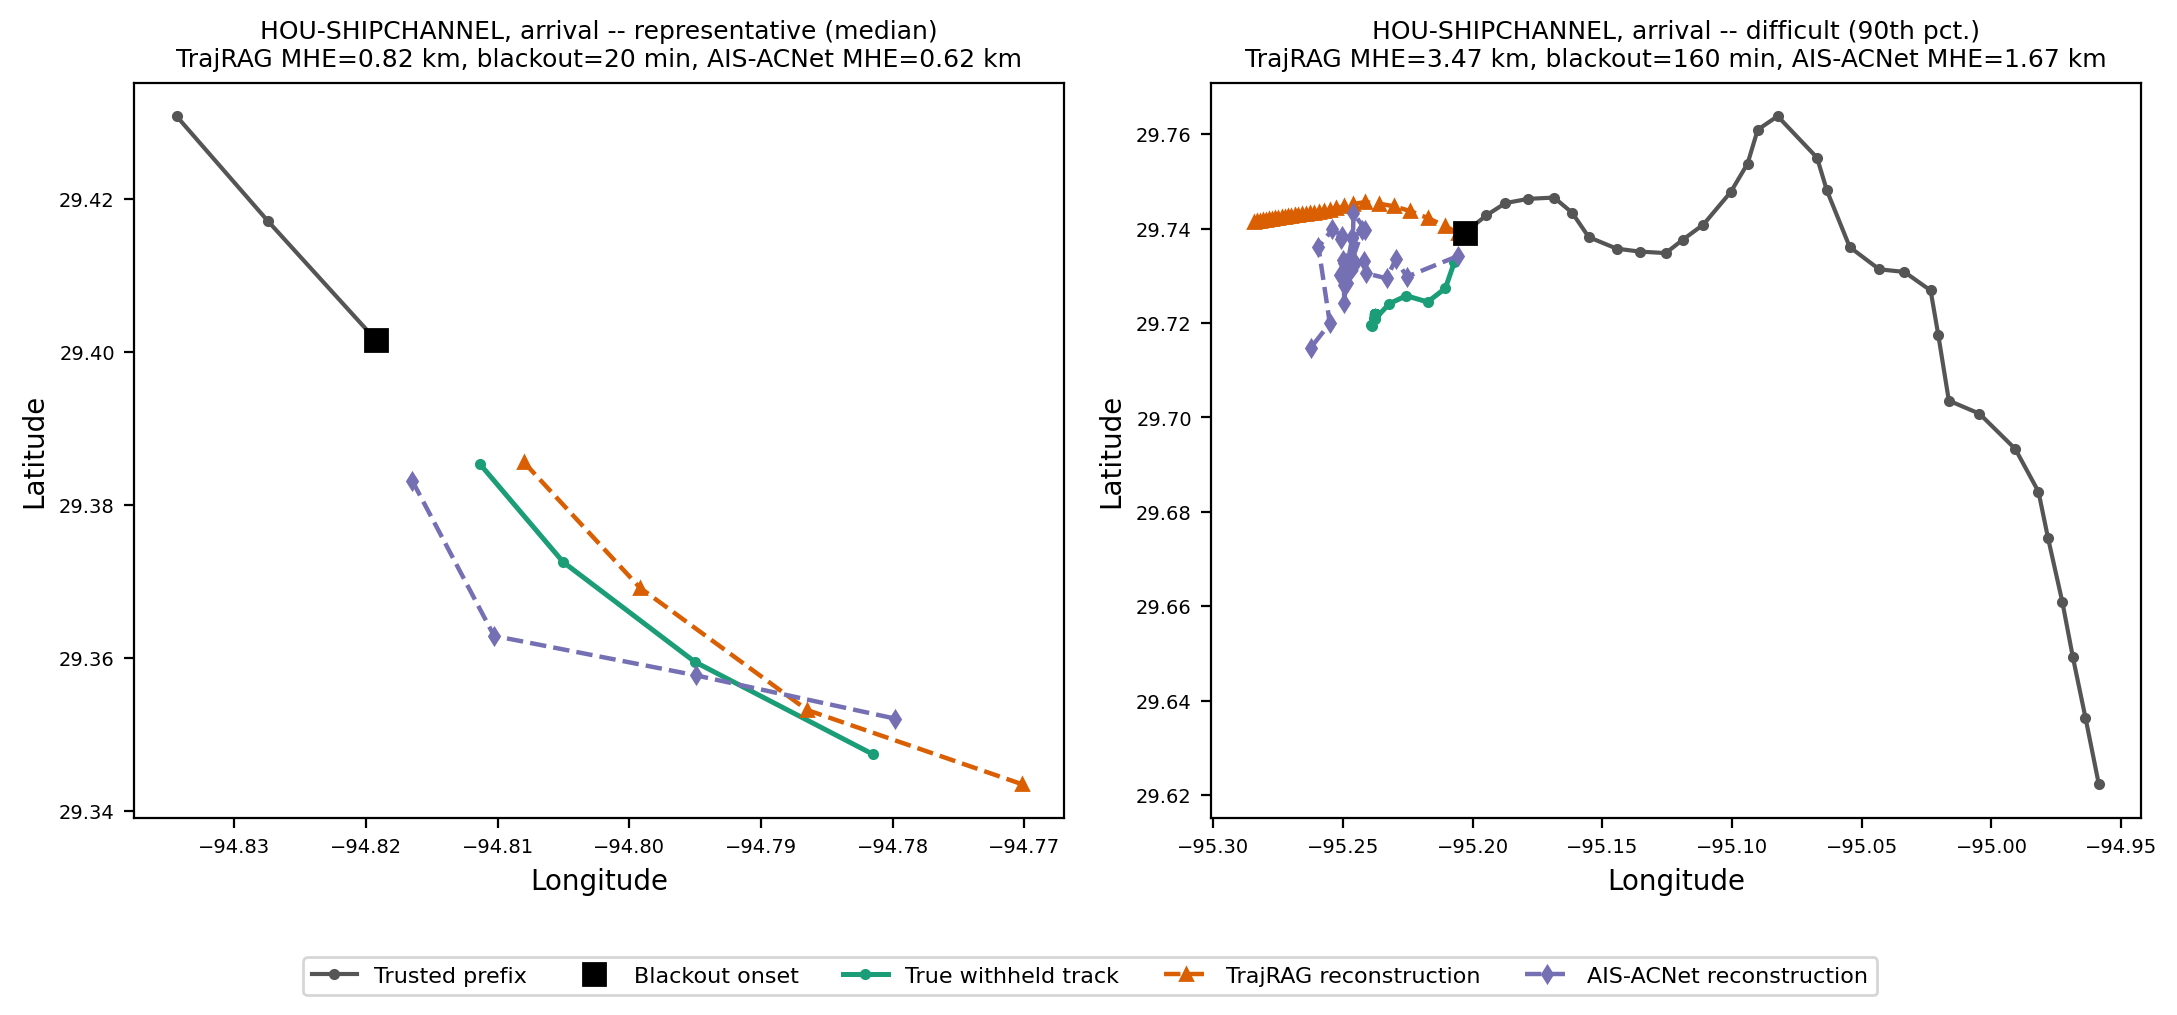
\includegraphics[width=\linewidth]{figures/case_houston_arrival.png}
\caption{Houston Ship Channel, arrival phase. Left: representative case
(voyage closest to the group median TrajRAG error, 0.82\,km, 20-minute
blackout). Right: difficult case (voyage closest to the group 90th
percentile, 3.47\,km, 160-minute blackout), where TrajRAG continues past
the true track's turn into the berth approach while AIS-ACNet oscillates
but stays closer to the true position -- an instance of the heavy right
tail noted in Section~\ref{sec:distribution}.}
\label{fig:case-houston}
\end{figure}

\begin{figure}[t]
\centering
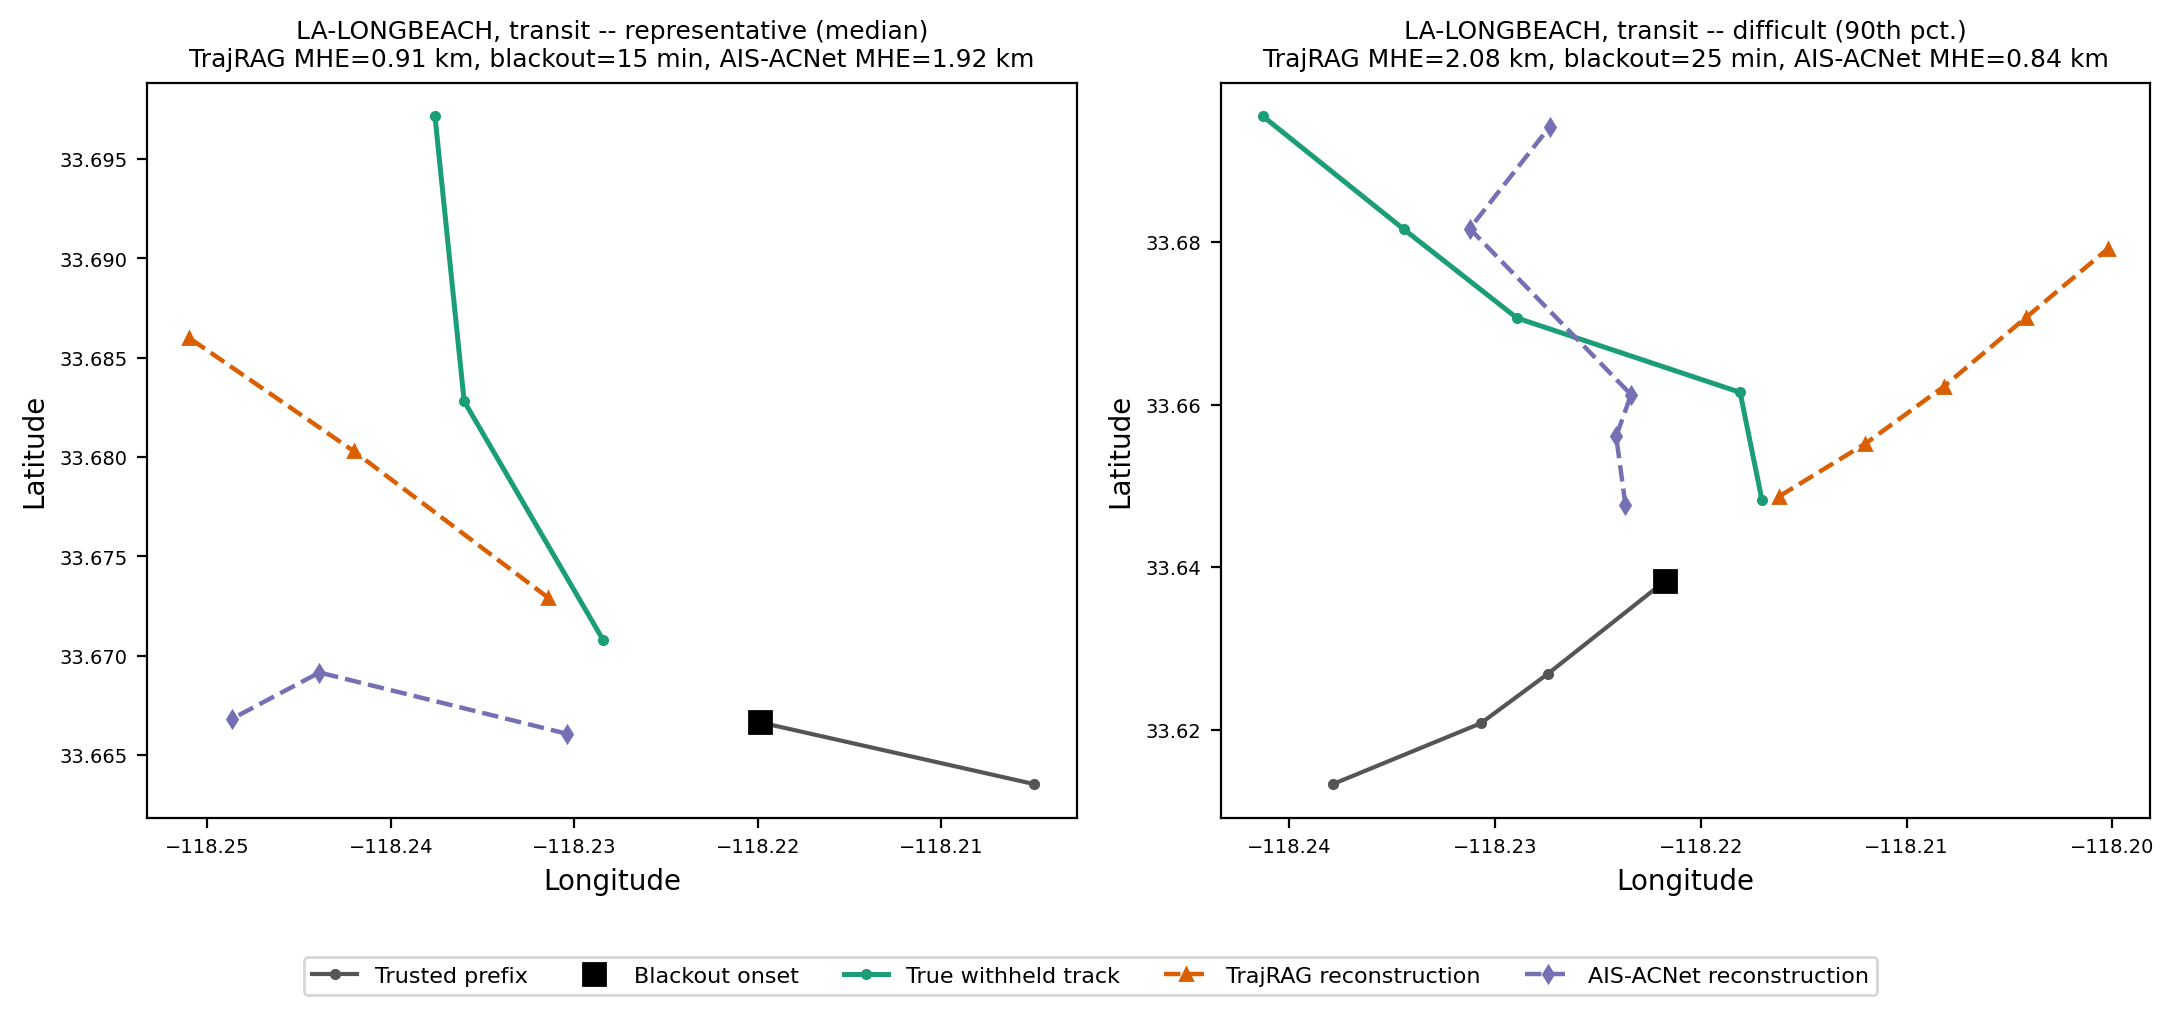
\includegraphics[width=\linewidth]{figures/case_la_transit.png}
\caption{Los Angeles/Long Beach, transit phase. Left: representative case
(0.91\,km TrajRAG error, 15-minute blackout), where TrajRAG tracks the true
withheld course more closely than AIS-ACNet. Right: difficult case
(2.08\,km TrajRAG error, 25-minute blackout), where AIS-ACNet's shorter,
more conservative reconstruction stays closer to the true track than
TrajRAG's. Together the two panels illustrate that neither method
dominates the other case by case, consistent with the non-significant
paired comparison for this corridor and phase (Table~\ref{tab:wilcoxon-la}).}
\label{fig:case-la}
\end{figure}

We do not mark guard interventions on these plots. Doing so would require
the raw, pre-clamp LLM proposal at each step of \emph{this specific}
reconstruction, which was not saved -- only the final accepted position
was. The no-guard ablation (Section~\ref{sec:maritime-ablations}) is not a
substitute: it is an independently sampled autoregressive run on a
different voyage subset, and because each step's prompt depends on the
accepted history so far, its predicted positions diverge from the guarded
run's from the first clamped step onward and cannot be aligned with it
step for step. Final accepted positions alone do not let us tell, after
the fact, which specific steps the guard clamped in the reconstructions
plotted here.
